\documentclass[aspectratio=169]{beamer}

\usepackage{ccicons}
\usepackage{fontspec}
\usepackage{import}
\usepackage{listings}
\usepackage{tikz}

\subimport{../}{colors.tex}

\usetikzlibrary{
  arrows,
  arrows.meta,
  automata,
  backgrounds,
  calc,
  chains,
  decorations.pathreplacing,
  fit,
  matrix,
  overlay-beamer-styles,
  positioning,
  shapes,
  tikzmark,
}
\usetikzmarklibrary{listings}

\hypersetup{
  colorlinks=true,
  urlcolor=uclablue,
}

\setbeamercolor{frametitle}{fg=primarycolor}
\setbeamercolor{structure}{fg=primarycolor}
\setbeamercolor{enumerate item}{fg=black}
\setbeamercolor{itemize item}{fg=black}
\setbeamercolor{itemize subitem}{fg=black}

\setbeamersize{text margin left=26.6mm}
\addtolength{\headsep}{2mm}

\setbeamertemplate{navigation symbols}{}
\setbeamertemplate{headline}{}
\setbeamertemplate{footline}{}
\setbeamertemplate{itemize item}{\color{black}}
\setbeamertemplate{itemize items}[circle]

\setbeamertemplate{footline}{
  \begin{tikzpicture}[remember picture,
                      overlay,
                      shift={(current page.south west)}]
    \node [black!50, inner sep=2mm, anchor=south east]
          at (current page.south east) {\footnotesize \insertframenumber};
  \end{tikzpicture}
}

\setsansfont{Overpass}[Scale=MatchLowercase]
\setmonofont{Overpass Mono}[Scale=MatchLowercase]

\makeatletter
\newcommand\version[1]{\renewcommand\@version{#1}}
\newcommand\@version{}
\def\insertversion{\@version}

\newcommand\lecturenumber[1]{\renewcommand\@lecturenumber{#1}}
\newcommand\@lecturenumber{}
\def\insertlecturenumber{\@lecturenumber}
\makeatother

\setbeamertemplate{title page}
{
  \begin{tikzpicture}[remember picture,
                      overlay,
                      shift={(current page.south west)},
                      background rectangle/.style={fill=uclablue},
                      show background rectangle]
    \node [anchor=west, align=left, inner sep=0, text=white]
          (lecturenumber) at (\paperwidth / 6, \paperheight * 3 / 4)
          {\Large Lecture \insertlecturenumber};
    \node [inner sep=0, align=left, text=white, node distance=0,
           above left=of lecturenumber, anchor=south west, yshift=2mm]
          {\Large CS 111: Operating System Principles};
    \node (title) [inner sep=0, anchor=west, align=right, text=white]
          at (\paperwidth / 6, \paperheight / 2)
          {{\bfseries \Huge \inserttitle{}}};
    \node [inner sep=0, align=right, text=white, node distance=0,
           below right=of title, anchor=north east, yshift=-1mm]
          {{\footnotesize \ttfamily \insertversion}};
    \node [inner sep=0, text=white, align=left, anchor=west]
          (author) at (\paperwidth / 6, \paperheight / 4)
          {\insertauthor};
    \node [text=white, inner sep=0, align=left, node distance=0,
           below left=of author, anchor=north west, yshift=-2mm]
          {\insertdate};
    \node [align=right, anchor=south east, inner sep=2mm, text=white]
          (license) at (\paperwidth, 0)
          {\footnotesize This  work is licensed under a
           \href{http://creativecommons.org/licenses/by-sa/4.0/}
                {\color{uclagold} Creative Commons Attribution-ShareAlike 4.0
                 International License}};
    \node [text=white, inner sep=0, align=right, node distance=0,
           above right=of license, anchor=south east, xshift=-2mm]
          {\Large \ccbysa};
  \end{tikzpicture}
}

\tikzset{
  >=Straight Barb[],
  shorten >=1pt,
  initial text=,
}

\lstset{
  basicstyle=\footnotesize\ttfamily,
}


\lecturenumber{7}
\title{Scheduling}
\version{2.0.1}
\author{Jon Eyolfson}
\date{July 13, 2021}

\begin{document}
  \begin{frame}[plain, noframenumbering]
    \titlepage
  \end{frame}

  \begin{frame}
    \frametitle{There are Preemptible and Non-preemptible Resources}

    A preemptible resource can be taken away and used for something else

    \hspace{2em} e.g. a CPU

    \vspace{2em}

    The resource is shared through scheduling

    \vspace{4em}

    A non-preemptible resource can not be taken away without acknowledgment

    \hspace{2em} e.g. disk space

    \vspace{2em}

    The resource is shared through allocations and deallocations

    \hspace{2em} Note: Parallel and distributed systems may allow you to allocate a CPU
  \end{frame}

  \begin{frame}
    \frametitle{A Dispatcher and Scheduler Work Together}

    A dispatcher is a low-level mechanism

    \hspace{2em} Responsible for context switching

    \vspace{2em}

    A scheduler is a high-level policy

    \hspace{2em} Responsible for deciding which processes to run
  \end{frame}

  \begin{frame}
    \frametitle{The Scheduler Runs Whenever a Process Changes State}

    First let's consider non-preemptable processes

    \hspace{2em} Once the process starts, it runs until completion

    \vspace{2em}

    In this case, the scheduler will only make a decision when the process
    terminates

    \vspace{4em}

    Preemptive allows the operating system to run the scheduler at will

    \hspace{2em} Check \texttt{uname -v}, your kernel should tell you it's preemptable
  \end{frame}

  \begin{frame}
    \frametitle{Metrics}

    Minimize waiting time and response time

    \hspace{2em} Don't have a process waiting too long (or too long to start)

    \vspace{2em}

    Maximize CPU utilization

    \hspace{2em} Don't have the CPU idle

    \vspace{2em}

    Maximize throughput

    \hspace{2em} Complete as many processes as possible

    \vspace{2em}

    Fairness

    \hspace{2em} Try to give each process the same percentage of the CPU
  \end{frame}

  \begin{frame}
    \frametitle{First Come First Served (FCFS)}

    The most basic form of scheduling

    \vspace{2em}

    The first process that arrives gets the CPU

    \vspace{2em}

    Processes are stored in a FIFO queue in arrival order
  \end{frame}
  
  \begin{frame}
    \frametitle{A Gantt Chart Illustrates the Schedule}

    Consider the following processes:
    \begin{center}
      \footnotesize
      \begin{tabular}{lrr}
        Process & Arrival Time & Burst Time \\
        $\mathsf{P_1}$ & 0 & 7 \\
        $\mathsf{P_2}$ & 0 & 4 \\
        $\mathsf{P_3}$ & 0 & 1 \\
        $\mathsf{P_4}$ & 0 & 4 \\
      \end{tabular}
    \end{center}

    Assume, $\mathsf{P_1} \rightarrow \mathsf{P_2} \rightarrow \mathsf{P_3}
             \rightarrow \mathsf{P_4}$.
    For FCFS, our schedule is:
    \begin{center}
      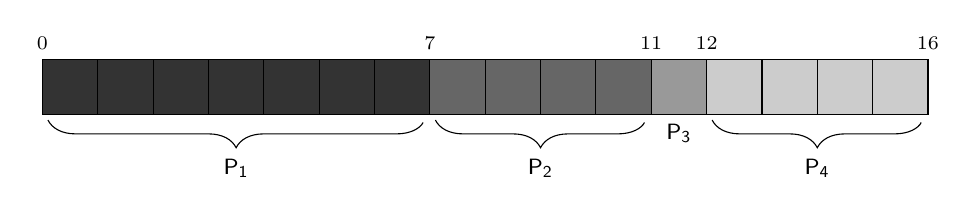
\begin{tikzpicture}

        \fill [black!80] (0,0) rectangle (14em, 2em);

        \fill [black!60] (14em,0) rectangle (22em, 2em);

        \fill [black!40] (22em,0) rectangle (24em, 2em);

        \fill [black!20] (24em,0) rectangle (32em, 2em);

        \draw (0,0) rectangle (32em,2em);

        \foreach \i in {1,...,15} {
          \draw [shorten >=0] (\i * 2em, 0) -- (\i * 2em, 2em);
        }

        \node [anchor=south] at (0em, 2em) {\scriptsize 0};
        \node [anchor=south] at (14em, 2em) {\scriptsize 7};
        \node [anchor=south] at (22em, 2em) {\scriptsize 11};
        \node [anchor=south] at (24em, 2em) {\scriptsize 12};
        \node [anchor=south] at (32em, 2em) {\scriptsize 16};

        \draw [decorate, decoration={brace,amplitude=10pt,mirror,raise=2pt}]
              (0.2em,0) -- (13.8em,0)
              node [midway, below, anchor=north, yshift=-1.25em]
              {\footnotesize $\mathsf{P_1}$};

        \draw [decorate, decoration={brace,amplitude=10pt,mirror,raise=2pt}]
              (14.2em,0) -- (21.8em,0)
              node [midway, below, anchor=north, yshift=-1.25em]
              {\footnotesize $\mathsf{P_2}$};

        \node [anchor=north] at (23em, 0) {\footnotesize $\mathsf{P_3}$};

        \draw [decorate, decoration={brace,amplitude=10pt,mirror,raise=2pt}]
              (24.2em,0) -- (31.8em,0)
              node [midway, below, anchor=north, yshift=-1.25em]
              {\footnotesize $\mathsf{P_4}$};
      \end{tikzpicture}
    \end{center}

    What is the average waiting time?
  \end{frame}
  
  \begin{frame}
    \frametitle{What Happens to Our Waiting Time with a Different Arrival Order}

    Consider the same processes:
    \begin{center}
      \footnotesize
      \begin{tabular}{lrr}
        Process & Arrival Time & Burst Time \\
        $\mathsf{P_1}$ & 0 & 7 \\
        $\mathsf{P_2}$ & 0 & 4 \\
        $\mathsf{P_3}$ & 0 & 1 \\
        $\mathsf{P_4}$ & 0 & 4 \\
      \end{tabular}
    \end{center}

    Assume, $\mathsf{P_3} \rightarrow \mathsf{P_2} \rightarrow \mathsf{P_4}
             \rightarrow \mathsf{P_1}$.
    For FCFS, our schedule is:
    \begin{center}
      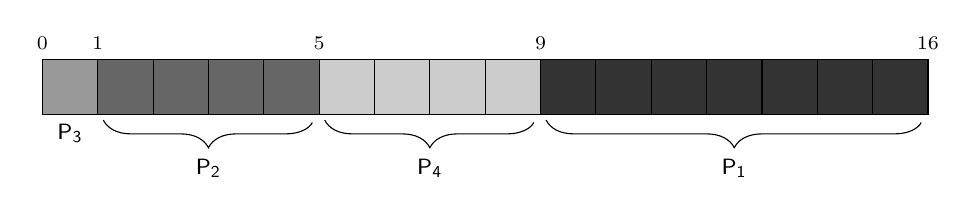
\begin{tikzpicture}

        \fill [black!80] (18em,0) rectangle (32em, 2em);

        \fill [black!60] (2em,0) rectangle (10em, 2em);

        \fill [black!40] (0em,0) rectangle (2em, 2em);

        \fill [black!20] (10em,0) rectangle (18em, 2em);

        \draw (0,0) rectangle (32em,2em);

        \foreach \i in {1,...,15} {
          \draw [shorten >=0] (\i * 2em, 0) -- (\i * 2em, 2em);
        }

        \node [anchor=south] at (0em, 2em) {\scriptsize 0};
        \node [anchor=south] at (2em, 2em) {\scriptsize 1};
        \node [anchor=south] at (10em, 2em) {\scriptsize 5};
        \node [anchor=south] at (18em, 2em) {\scriptsize 9};
        \node [anchor=south] at (32em, 2em) {\scriptsize 16};

        \node [anchor=north] at (1em, 0) {\footnotesize $\mathsf{P_3}$};

        \draw [decorate, decoration={brace,amplitude=10pt,mirror,raise=2pt}]
              (18.2em,0) -- (31.8em,0)
              node [midway, below, anchor=north, yshift=-1.25em]
              {\footnotesize $\mathsf{P_1}$};

        \draw [decorate, decoration={brace,amplitude=10pt,mirror,raise=2pt}]
              (2.2em,0) -- (9.8em,0)
              node [midway, below, anchor=north, yshift=-1.25em]
              {\footnotesize $\mathsf{P_2}$};

        \draw [decorate, decoration={brace,amplitude=10pt,mirror,raise=2pt}]
              (10.2em,0) -- (17.8em,0)
              node [midway, below, anchor=north, yshift=-1.25em]
              {\footnotesize $\mathsf{P_4}$};
      \end{tikzpicture}
    \end{center}

    What is the average waiting time now?
  \end{frame}

  \begin{frame}
    \frametitle{Shortest Job First (SJF)}

    A slight tweak to FCFS, we always schedule the job with the shortest burst time
    first

    \vspace{2em}

    We're still assuming no preemption
  \end{frame}

  \begin{frame}
    \frametitle{SJF Minimizes the Average Wait Time over FCFS}

    Consider the same processes with different arrival times:
    \begin{center}
      \footnotesize
      \begin{tabular}{lrr}
        Process & Arrival Time & Burst Time \\
        $\mathsf{P_1}$ & 0 & 7 \\
        $\mathsf{P_2}$ & 2 & 4 \\
        $\mathsf{P_3}$ & 4 & 1 \\
        $\mathsf{P_4}$ & 5 & 4 \\
      \end{tabular}
    \end{center}

    For SJF, our schedule is (arrival on top):
    \begin{center}
      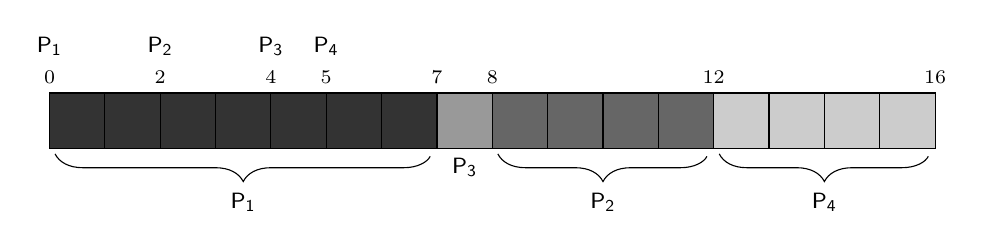
\begin{tikzpicture}

        \fill [black!80] (0,0) rectangle (14em, 2em);

        \fill [black!60] (16em,0) rectangle (24em, 2em);

        \fill [black!40] (14em,0) rectangle (16em, 2em);

        \fill [black!20] (24em,0) rectangle (32em, 2em);

        \draw (0,0) rectangle (32em,2em);

        \foreach \i in {1,...,15} {
          \draw [shorten >=0] (\i * 2em, 0) -- (\i * 2em, 2em);
        }

        \node [anchor=south] at (0em, 2em) {\scriptsize 0};
        \node [anchor=south] at (4em, 2em) {\scriptsize 2};
        \node [anchor=south] at (8em, 2em) {\scriptsize 4};
        \node [anchor=south] at (10em, 2em) {\scriptsize 5};
        \node [anchor=south] at (14em, 2em) {\scriptsize 7};
        \node [anchor=south] at (16em, 2em) {\scriptsize 8};
        \node [anchor=south] at (24em, 2em) {\scriptsize 12};
        \node [anchor=south] at (32em, 2em) {\scriptsize 16};

        \draw [decorate, decoration={brace,amplitude=10pt,mirror,raise=2pt}]
              (0.2em,0) -- (13.8em,0)
              node [midway, below, anchor=north, yshift=-1.25em]
              {\footnotesize $\mathsf{P_1}$};

        \draw [decorate, decoration={brace,amplitude=10pt,mirror,raise=2pt}]
              (16.2em,0) -- (23.8em,0)
              node [midway, below, anchor=north, yshift=-1.25em]
              {\footnotesize $\mathsf{P_2}$};

        \node [anchor=north] at (15em, 0) {\footnotesize $\mathsf{P_3}$};

        \draw [decorate, decoration={brace,amplitude=10pt,mirror,raise=2pt}]
              (24.2em,0) -- (31.8em,0)
              node [midway, below, anchor=north, yshift=-1.25em]
              {\footnotesize $\mathsf{P_4}$};

        \node [anchor=south, yshift=1em] at (0em, 2em) {\footnotesize $\mathsf{P_1}$};

        \node [anchor=south, yshift=1em] at (4em, 2em) {\footnotesize $\mathsf{P_2}$};

        \node [anchor=south, yshift=1em] at (8em, 2em) {\footnotesize $\mathsf{P_3}$};

        \node [anchor=south, yshift=1em] at (10em, 2em) {\footnotesize $\mathsf{P_4}$};
      \end{tikzpicture}
    \end{center}

    Average waiting time: $\mathsf{\frac{0 + 6 + 3 + 7}{4} = 4}$
  \end{frame}

  \begin{frame}
    \frametitle{SJF is Not Practical}

    It is provably optimal at minimizing average wait time (if no preemption)

    \vspace{2em}

    You will not know the burst times of each process

    \hspace{2em} You could use the past to predict future executions

    \vspace{2em}

    You may starve long jobs (they may never execute)
  \end{frame}

  \begin{frame}
    \frametitle{Shortest Remaining Time First (SRTF)}

    Changing SJF to run with preemptions requires another tweak

    \vspace{2em}

    We'll assume that our minimum execution time is one unit

    \vspace{2em}

    Similar to SJF, this optimizes the average waiting time
  \end{frame}

  \begin{frame}
    \frametitle{SRTF Reduces the Average Wait Time Compared to SJF}

    Consider the same processes and arrival times as SJF:
    \begin{center}
      \footnotesize
      \begin{tabular}{lrr}
        Process & Arrival Time & Burst Time \\
        $\mathsf{P_1}$ & 0 & 7 \\
        $\mathsf{P_2}$ & 2 & 4 \\
        $\mathsf{P_3}$ & 4 & 1 \\
        $\mathsf{P_4}$ & 5 & 4 \\
      \end{tabular}
    \end{center}

    For SRTF, our schedule is (arrival on top):
    \begin{center}
      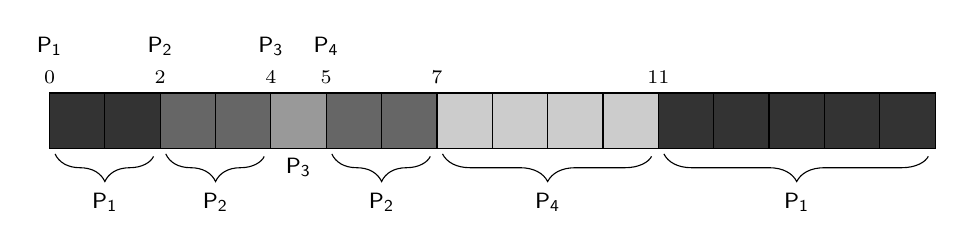
\begin{tikzpicture}

        \fill [black!80] (0,0) rectangle (4em, 2em);

        \fill [black!60] (4em,0) rectangle (8em, 2em);

        \fill [black!40] (8em,0) rectangle (10em, 2em);

        \fill [black!60] (10em,0) rectangle (14em, 2em);

        \fill [black!20] (14em,0) rectangle (22em, 2em);

        \fill [black!80] (22em,0) rectangle (32em, 2em);

        \draw (0,0) rectangle (32em,2em);

        \foreach \i in {1,...,15} {
          \draw [shorten >=0] (\i * 2em, 0) -- (\i * 2em, 2em);
        }

        \node [anchor=south] at (0em, 2em) {\scriptsize 0};
        \node [anchor=south] at (4em, 2em) {\scriptsize 2};
        \node [anchor=south] at (8em, 2em) {\scriptsize 4};
        \node [anchor=south] at (10em, 2em) {\scriptsize 5};
        \node [anchor=south] at (14em, 2em) {\scriptsize 7};
        \node [anchor=south] at (22em, 2em) {\scriptsize 11};

        \draw [decorate, decoration={brace,amplitude=10pt,mirror,raise=2pt}]
              (0.2em,0) -- (3.8em,0)
              node [midway, below, anchor=north, yshift=-1.25em]
              {\footnotesize $\mathsf{P_1}$};

        \draw [decorate, decoration={brace,amplitude=10pt,mirror,raise=2pt}]
              (4.2em,0) -- (7.8em,0)
              node [midway, below, anchor=north, yshift=-1.25em]
              {\footnotesize $\mathsf{P_2}$};

        \node [anchor=north] at (9em, 0) {\footnotesize $\mathsf{P_3}$};

        \draw [decorate, decoration={brace,amplitude=10pt,mirror,raise=2pt}]
              (10.2em,0) -- (13.8em,0)
              node [midway, below, anchor=north, yshift=-1.25em]
              {\footnotesize $\mathsf{P_2}$};

        \draw [decorate, decoration={brace,amplitude=10pt,mirror,raise=2pt}]
              (14.2em,0) -- (21.8em,0)
              node [midway, below, anchor=north, yshift=-1.25em]
              {\footnotesize $\mathsf{P_4}$};
              
        \draw [decorate, decoration={brace,amplitude=10pt,mirror,raise=2pt}]
              (22.2em,0) -- (31.8em,0)
              node [midway, below, anchor=north, yshift=-1.25em]
              {\footnotesize $\mathsf{P_1}$};

        \node [anchor=south, yshift=1em] at (0em, 2em) {\footnotesize $\mathsf{P_1}$};

        \node [anchor=south, yshift=1em] at (4em, 2em) {\footnotesize $\mathsf{P_2}$};

        \node [anchor=south, yshift=1em] at (8em, 2em) {\footnotesize $\mathsf{P_3}$};

        \node [anchor=south, yshift=1em] at (10em, 2em) {\footnotesize $\mathsf{P_4}$};
      \end{tikzpicture}
    \end{center}

    Average waiting time: $\mathsf{\frac{9 + 1 + 0 + 2}{4} = 3}$
  \end{frame}

  \begin{frame}
    \frametitle{Round-Robin (RR)}

    So far we haven't handled fairness (it's a trade off with other metrics)

    \vspace{2em}

    The operating system divides execution into time slices (or quanta)

    \hspace{2em} An individual time slice is called a quantum

    \vspace{2em}

    Maintain a FIFO queue of processes similar to FCFS

    \hspace{2em} Preempt if still running at end of quantum and re-add to queue

    \vspace{2em}

    What are practical considerations for determining quantum length?
  \end{frame}

  \begin{frame}
    \frametitle{RR with a Quantum Length of 3 Units}

    \begin{center}
      \footnotesize
      \begin{tabular}{lrr}
        Process & Arrival Time & Burst Time \\
        $\mathsf{P_1}$ & 0 & 7 \\
        $\mathsf{P_2}$ & 2 & 4 \\
        $\mathsf{P_3}$ & 4 & 1 \\
        $\mathsf{P_4}$ & 5 & 4 \\
      \end{tabular}
    \end{center}

    For RR, our schedule is (arrival on top, queue on bottom):
    \begin{center}
      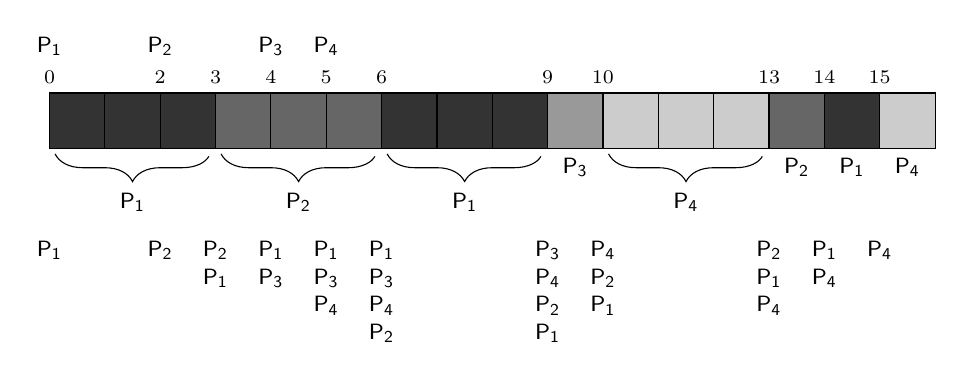
\begin{tikzpicture}

        \fill [black!80] (0,0) rectangle (6em, 2em);
        
        \fill [black!60] (6em,0) rectangle (12em, 2em);

        \fill [black!80] (12em,0) rectangle (18em, 2em);

        \fill [black!40] (18em,0) rectangle (20em, 2em);

        \fill [black!20] (20em,0) rectangle (26em, 2em);

        \fill [black!60] (26em,0) rectangle (28em, 2em);

        \fill [black!80] (28em,0) rectangle (30em, 2em);

        \fill [black!20] (30em,0) rectangle (32em, 2em);

        \draw (0,0) rectangle (32em,2em);

        \foreach \i in {1,...,15} {
          \draw [shorten >=0] (\i * 2em, 0) -- (\i * 2em, 2em);
        }

        \node [anchor=south] at (0em, 2em) {\scriptsize 0};
        \node [anchor=south] at (4em, 2em) {\scriptsize 2};
        \node [anchor=south] at (6em, 2em) {\scriptsize 3};
        \node [anchor=south] at (8em, 2em) {\scriptsize 4};
        \node [anchor=south] at (10em, 2em) {\scriptsize 5};
        \node [anchor=south] at (12em, 2em) {\scriptsize 6};
        \node [anchor=south] at (18em, 2em) {\scriptsize 9};
        \node [anchor=south] at (20em, 2em) {\scriptsize 10};
        \node [anchor=south] at (26em, 2em) {\scriptsize 13};
        \node [anchor=south] at (28em, 2em) {\scriptsize 14};
        \node [anchor=south] at (30em, 2em) {\scriptsize 15};

        \draw [decorate, decoration={brace,amplitude=10pt,mirror,raise=2pt}]
              (0.2em,0) -- (5.8em,0)
              node [midway, below, anchor=north, yshift=-1.25em]
              {\footnotesize $\mathsf{P_1}$};

        \draw [decorate, decoration={brace,amplitude=10pt,mirror,raise=2pt}]
              (6.2em,0) -- (11.8em,0)
              node [midway, below, anchor=north, yshift=-1.25em]
              {\footnotesize $\mathsf{P_2}$};

        \draw [decorate, decoration={brace,amplitude=10pt,mirror,raise=2pt}]
              (12.2em,0) -- (17.8em,0)
              node [midway, below, anchor=north, yshift=-1.25em]
              {\footnotesize $\mathsf{P_1}$};

        \node [anchor=north] at (19em, 0) {\footnotesize $\mathsf{P_3}$};

        \draw [decorate, decoration={brace,amplitude=10pt,mirror,raise=2pt}]
              (20.2em,0) -- (25.8em,0)
              node [midway, below, anchor=north, yshift=-1.25em]
              {\footnotesize $\mathsf{P_4}$};

        \node [anchor=north] at (27em, 0) {\footnotesize $\mathsf{P_2}$};

        \node [anchor=north] at (29em, 0) {\footnotesize $\mathsf{P_1}$};

        \node [anchor=north] at (31em, 0) {\footnotesize $\mathsf{P_4}$};

        \node [anchor=south, yshift=1em] at (0em, 2em) {\footnotesize $\mathsf{P_1}$};

        \node [anchor=south, yshift=1em] at (4em, 2em) {\footnotesize $\mathsf{P_2}$};

        \node [anchor=south, yshift=1em] at (8em, 2em) {\footnotesize $\mathsf{P_3}$};

        \node [anchor=south, yshift=1em] at (10em, 2em) {\footnotesize $\mathsf{P_4}$};

        \node [anchor=north, yshift=-3em] at (0em, 0em) {\footnotesize $\mathsf{P_1}$};

        \node [anchor=north, yshift=-3em] at (4em, 0em) {\footnotesize $\mathsf{P_2}$};

        \node [anchor=north, yshift=-3em] at (6em, 0em) {\footnotesize $\mathsf{P_2}$};
        \node [anchor=north, yshift=-4em] at (6em, 0em) {\footnotesize $\mathsf{P_1}$};

        \node [anchor=north, yshift=-3em] at (8em, 0em) {\footnotesize $\mathsf{P_1}$};
        \node [anchor=north, yshift=-4em] at (8em, 0em) {\footnotesize $\mathsf{P_3}$};

        \node [anchor=north, yshift=-3em] at (10em, 0em) {\footnotesize $\mathsf{P_1}$};
        \node [anchor=north, yshift=-4em] at (10em, 0em) {\footnotesize $\mathsf{P_3}$};
        \node [anchor=north, yshift=-5em] at (10em, 0em) {\footnotesize $\mathsf{P_4}$};

        \node [anchor=north, yshift=-3em] at (12em, 0em) {\footnotesize $\mathsf{P_1}$};
        \node [anchor=north, yshift=-4em] at (12em, 0em) {\footnotesize $\mathsf{P_3}$};
        \node [anchor=north, yshift=-5em] at (12em, 0em) {\footnotesize $\mathsf{P_4}$};
        \node [anchor=north, yshift=-6em] at (12em, 0em) {\footnotesize $\mathsf{P_2}$};

        \node [anchor=north, yshift=-3em] at (18em, 0em) {\footnotesize $\mathsf{P_3}$};
        \node [anchor=north, yshift=-4em] at (18em, 0em) {\footnotesize $\mathsf{P_4}$};
        \node [anchor=north, yshift=-5em] at (18em, 0em) {\footnotesize $\mathsf{P_2}$};
        \node [anchor=north, yshift=-6em] at (18em, 0em) {\footnotesize $\mathsf{P_1}$};

        \node [anchor=north, yshift=-3em] at (20em, 0em) {\footnotesize $\mathsf{P_4}$};
        \node [anchor=north, yshift=-4em] at (20em, 0em) {\footnotesize $\mathsf{P_2}$};
        \node [anchor=north, yshift=-5em] at (20em, 0em) {\footnotesize $\mathsf{P_1}$};

        \node [anchor=north, yshift=-3em] at (26em, 0em) {\footnotesize $\mathsf{P_2}$};
        \node [anchor=north, yshift=-4em] at (26em, 0em) {\footnotesize $\mathsf{P_1}$};
        \node [anchor=north, yshift=-5em] at (26em, 0em) {\footnotesize $\mathsf{P_4}$};

        \node [anchor=north, yshift=-3em] at (28em, 0em) {\footnotesize $\mathsf{P_1}$};
        \node [anchor=north, yshift=-4em] at (28em, 0em) {\footnotesize $\mathsf{P_4}$};

        \node [anchor=north, yshift=-3em] at (30em, 0em) {\footnotesize $\mathsf{P_4}$};
      \end{tikzpicture}
    \end{center}
  \end{frame}

  \begin{frame}
    \frametitle{Metrics for RR (3 Unit Quantum Length)}

    Number of context switches: 7

    \vspace{2em}

    Average waiting time: $\mathsf{\frac{8 + 8 + 5 + 7}{4} = 7}$

    \vspace{2em}

    Average response time: $\mathsf{\frac{0 + 1 + 5 + 5}{4} = 2.75}$

    \vspace{4em}

    Note: on ties (a new process arrives while one is preempted), favor the new one
  \end{frame}

  \begin{frame}
    \frametitle{RR with a Quantum Length of 1 Units}

    \begin{center}
      \footnotesize
      \begin{tabular}{lrr}
        Process & Arrival Time & Burst Time \\
        $\mathsf{P_1}$ & 0 & 7 \\
        $\mathsf{P_2}$ & 2 & 4 \\
        $\mathsf{P_3}$ & 4 & 1 \\
        $\mathsf{P_4}$ & 5 & 4 \\
      \end{tabular}
    \end{center}

    For RR, our schedule is (arrival on top, queue on bottom):
    \begin{center}
      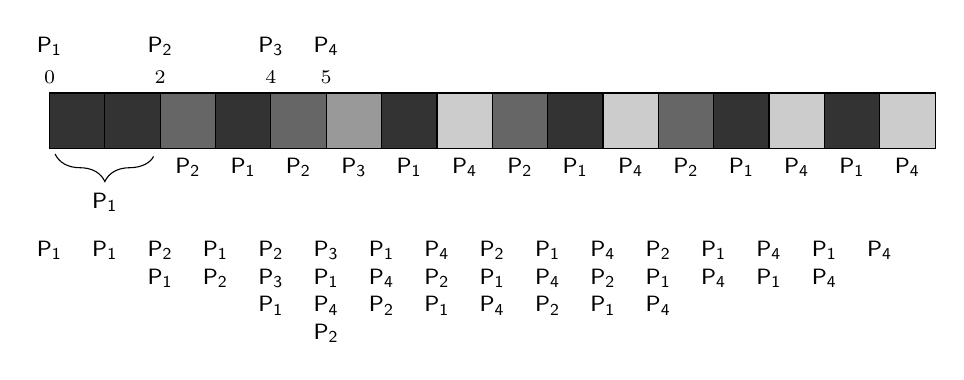
\begin{tikzpicture}

        \fill [black!80] (0,0) rectangle (4em, 2em);
        \fill [black!60] (4em,0) rectangle (6em, 2em);
        \fill [black!80] (6em,0) rectangle (8em, 2em);
        \fill [black!60] (8em,0) rectangle (10em, 2em);
        \fill [black!40] (10em,0) rectangle (12em, 2em);
        \fill [black!80] (12em,0) rectangle (14em, 2em);
        \fill [black!20] (14em,0) rectangle (16em, 2em);
        \fill [black!60] (16em,0) rectangle (18em, 2em);
        \fill [black!80] (18em,0) rectangle (20em, 2em);
        \fill [black!20] (20em,0) rectangle (22em, 2em);
        \fill [black!60] (22em,0) rectangle (24em, 2em);
        \fill [black!80] (24em,0) rectangle (26em, 2em);
        \fill [black!20] (26em,0) rectangle (28em, 2em);
        \fill [black!80] (28em,0) rectangle (30em, 2em);
        \fill [black!20] (30em,0) rectangle (32em, 2em);

        \draw (0,0) rectangle (32em,2em);

        \foreach \i in {1,...,15} {
          \draw [shorten >=0] (\i * 2em, 0) -- (\i * 2em, 2em);
        }

        \node [anchor=south] at (0em, 2em) {\scriptsize 0};
        \node [anchor=south] at (4em, 2em) {\scriptsize 2};
        \node [anchor=south] at (8em, 2em) {\scriptsize 4};
        \node [anchor=south] at (10em, 2em) {\scriptsize 5};

        \draw [decorate, decoration={brace,amplitude=10pt,mirror,raise=2pt}]
              (0.2em,0) -- (3.8em,0)
              node [midway, below, anchor=north, yshift=-1.25em]
              {\footnotesize $\mathsf{P_1}$};

        \node [anchor=north] at (5em, 0) {\footnotesize $\mathsf{P_2}$};
        \node [anchor=north] at (7em, 0) {\footnotesize $\mathsf{P_1}$};
        \node [anchor=north] at (9em, 0) {\footnotesize $\mathsf{P_2}$};
        \node [anchor=north] at (11em, 0) {\footnotesize $\mathsf{P_3}$};
        \node [anchor=north] at (13em, 0) {\footnotesize $\mathsf{P_1}$};
        \node [anchor=north] at (15em, 0) {\footnotesize $\mathsf{P_4}$};
        \node [anchor=north] at (17em, 0) {\footnotesize $\mathsf{P_2}$};
        \node [anchor=north] at (19em, 0) {\footnotesize $\mathsf{P_1}$};
        \node [anchor=north] at (21em, 0) {\footnotesize $\mathsf{P_4}$};
        \node [anchor=north] at (23em, 0) {\footnotesize $\mathsf{P_2}$};
        \node [anchor=north] at (25em, 0) {\footnotesize $\mathsf{P_1}$};
        \node [anchor=north] at (27em, 0) {\footnotesize $\mathsf{P_4}$};
        \node [anchor=north] at (29em, 0) {\footnotesize $\mathsf{P_1}$};
        \node [anchor=north] at (31em, 0) {\footnotesize $\mathsf{P_4}$};

        % Arrivals
        \node [anchor=south, yshift=1em] at (0em, 2em) {\footnotesize $\mathsf{P_1}$};
        \node [anchor=south, yshift=1em] at (4em, 2em) {\footnotesize $\mathsf{P_2}$};
        \node [anchor=south, yshift=1em] at (8em, 2em) {\footnotesize $\mathsf{P_3}$};
        \node [anchor=south, yshift=1em] at (10em, 2em) {\footnotesize $\mathsf{P_4}$};

        % Queues
        \node [anchor=north, yshift=-3em] at (0em, 0em) {\footnotesize $\mathsf{P_1}$};

        \node [anchor=north, yshift=-3em] at (2em, 0em) {\footnotesize $\mathsf{P_1}$};

        \node [anchor=north, yshift=-3em] at (4em, 0em) {\footnotesize $\mathsf{P_2}$};
        \node [anchor=north, yshift=-4em] at (4em, 0em) {\footnotesize $\mathsf{P_1}$};

        \node [anchor=north, yshift=-3em] at (6em, 0em) {\footnotesize $\mathsf{P_1}$};
        \node [anchor=north, yshift=-4em] at (6em, 0em) {\footnotesize $\mathsf{P_2}$};

        \node [anchor=north, yshift=-3em] at (8em, 0em) {\footnotesize $\mathsf{P_2}$};
        \node [anchor=north, yshift=-4em] at (8em, 0em) {\footnotesize $\mathsf{P_3}$};
        \node [anchor=north, yshift=-5em] at (8em, 0em) {\footnotesize $\mathsf{P_1}$};

        \node [anchor=north, yshift=-3em] at (10em, 0em) {\footnotesize $\mathsf{P_3}$};
        \node [anchor=north, yshift=-4em] at (10em, 0em) {\footnotesize $\mathsf{P_1}$};
        \node [anchor=north, yshift=-5em] at (10em, 0em) {\footnotesize $\mathsf{P_4}$};
        \node [anchor=north, yshift=-6em] at (10em, 0em) {\footnotesize $\mathsf{P_2}$};

        \node [anchor=north, yshift=-3em] at (12em, 0em) {\footnotesize $\mathsf{P_1}$};
        \node [anchor=north, yshift=-4em] at (12em, 0em) {\footnotesize $\mathsf{P_4}$};
        \node [anchor=north, yshift=-5em] at (12em, 0em) {\footnotesize $\mathsf{P_2}$};

        \node [anchor=north, yshift=-3em] at (14em, 0em) {\footnotesize $\mathsf{P_4}$};
        \node [anchor=north, yshift=-4em] at (14em, 0em) {\footnotesize $\mathsf{P_2}$};
        \node [anchor=north, yshift=-5em] at (14em, 0em) {\footnotesize $\mathsf{P_1}$};

        \node [anchor=north, yshift=-3em] at (16em, 0em) {\footnotesize $\mathsf{P_2}$};
        \node [anchor=north, yshift=-4em] at (16em, 0em) {\footnotesize $\mathsf{P_1}$};
        \node [anchor=north, yshift=-5em] at (16em, 0em) {\footnotesize $\mathsf{P_4}$};

        \node [anchor=north, yshift=-3em] at (18em, 0em) {\footnotesize $\mathsf{P_1}$};
        \node [anchor=north, yshift=-4em] at (18em, 0em) {\footnotesize $\mathsf{P_4}$};
        \node [anchor=north, yshift=-5em] at (18em, 0em) {\footnotesize $\mathsf{P_2}$};

        \node [anchor=north, yshift=-3em] at (20em, 0em) {\footnotesize $\mathsf{P_4}$};
        \node [anchor=north, yshift=-4em] at (20em, 0em) {\footnotesize $\mathsf{P_2}$};
        \node [anchor=north, yshift=-5em] at (20em, 0em) {\footnotesize $\mathsf{P_1}$};

        \node [anchor=north, yshift=-3em] at (22em, 0em) {\footnotesize $\mathsf{P_2}$};
        \node [anchor=north, yshift=-4em] at (22em, 0em) {\footnotesize $\mathsf{P_1}$};
        \node [anchor=north, yshift=-5em] at (22em, 0em) {\footnotesize $\mathsf{P_4}$};

        \node [anchor=north, yshift=-3em] at (24em, 0em) {\footnotesize $\mathsf{P_1}$};
        \node [anchor=north, yshift=-4em] at (24em, 0em) {\footnotesize $\mathsf{P_4}$};

        \node [anchor=north, yshift=-3em] at (26em, 0em) {\footnotesize $\mathsf{P_4}$};
        \node [anchor=north, yshift=-4em] at (26em, 0em) {\footnotesize $\mathsf{P_1}$};

        \node [anchor=north, yshift=-3em] at (28em, 0em) {\footnotesize $\mathsf{P_1}$};
        \node [anchor=north, yshift=-4em] at (28em, 0em) {\footnotesize $\mathsf{P_4}$};

        \node [anchor=north, yshift=-3em] at (30em, 0em) {\footnotesize $\mathsf{P_4}$};
      \end{tikzpicture}
    \end{center}
  \end{frame}

  \begin{frame}
    \frametitle{Metrics for RR (1 Unit Quantum Length)}

    Number of context switches: 14

    \vspace{2em}

    Average waiting time: $\mathsf{\frac{8 + 6 + 1 + 7}{4} = 5.5}$

    \vspace{2em}

    Average response time: $\mathsf{\frac{0 + 0 + 1 + 2}{4} = 0.75}$
  \end{frame}

  \begin{frame}
    \frametitle{RR with a Quantum Length of 10 Units}

    \begin{center}
      \footnotesize
      \begin{tabular}{lrr}
        Process & Arrival Time & Burst Time \\
        $\mathsf{P_1}$ & 0 & 7 \\
        $\mathsf{P_2}$ & 2 & 4 \\
        $\mathsf{P_3}$ & 4 & 1 \\
        $\mathsf{P_4}$ & 5 & 4 \\
      \end{tabular}
    \end{center}

    For RR, our schedule is (arrival on top, queue on bottom):

    \begin{center}
      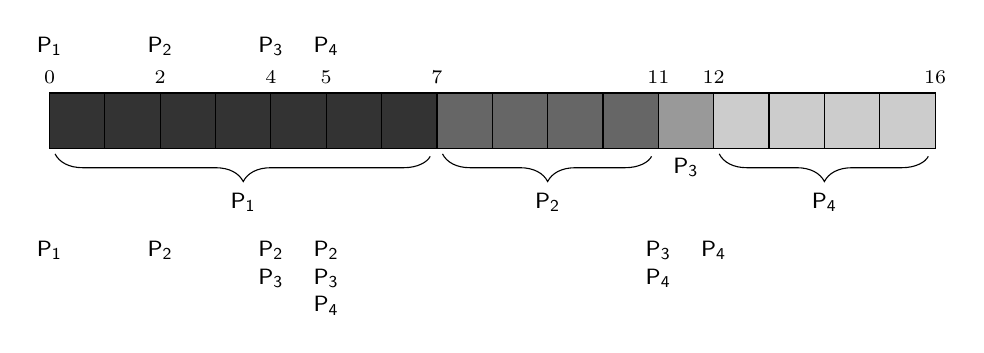
\begin{tikzpicture}

        \fill [black!80] (0,0) rectangle (14em, 2em);

        \fill [black!60] (14em,0) rectangle (22em, 2em);

        \fill [black!40] (22em,0) rectangle (24em, 2em);

        \fill [black!20] (24em,0) rectangle (32em, 2em);

        \draw (0,0) rectangle (32em,2em);

        \foreach \i in {1,...,15} {
          \draw [shorten >=0] (\i * 2em, 0) -- (\i * 2em, 2em);
        }

        \node [anchor=south] at (0em, 2em) {\scriptsize 0};
        \node [anchor=south] at (4em, 2em) {\scriptsize 2};
        \node [anchor=south] at (8em, 2em) {\scriptsize 4};
        \node [anchor=south] at (10em, 2em) {\scriptsize 5};
        \node [anchor=south] at (14em, 2em) {\scriptsize 7};
        \node [anchor=south] at (22em, 2em) {\scriptsize 11};
        \node [anchor=south] at (24em, 2em) {\scriptsize 12};
        \node [anchor=south] at (32em, 2em) {\scriptsize 16};

        % Arrivals
        \node [anchor=south, yshift=1em] at (0em, 2em) {\footnotesize $\mathsf{P_1}$};
        \node [anchor=south, yshift=1em] at (4em, 2em) {\footnotesize $\mathsf{P_2}$};
        \node [anchor=south, yshift=1em] at (8em, 2em) {\footnotesize $\mathsf{P_3}$};
        \node [anchor=south, yshift=1em] at (10em, 2em) {\footnotesize $\mathsf{P_4}$};

        % Queues
        \node [anchor=north, yshift=-3em] at (0em, 0em) {\footnotesize $\mathsf{P_1}$};

        \node [anchor=north, yshift=-3em] at (4em, 0em) {\footnotesize $\mathsf{P_2}$};

        \node [anchor=north, yshift=-3em] at (8em, 0em) {\footnotesize $\mathsf{P_2}$};
        \node [anchor=north, yshift=-4em] at (8em, 0em) {\footnotesize $\mathsf{P_3}$};

        \node [anchor=north, yshift=-3em] at (10em, 0em) {\footnotesize $\mathsf{P_2}$};
        \node [anchor=north, yshift=-4em] at (10em, 0em) {\footnotesize $\mathsf{P_3}$};
        \node [anchor=north, yshift=-5em] at (10em, 0em) {\footnotesize $\mathsf{P_4}$};

        \node [anchor=north, yshift=-3em] at (22em, 0em) {\footnotesize $\mathsf{P_3}$};
        \node [anchor=north, yshift=-4em] at (22em, 0em) {\footnotesize $\mathsf{P_4}$};

        \node [anchor=north, yshift=-3em] at (24em, 0em) {\footnotesize $\mathsf{P_4}$};


        \draw [decorate, decoration={brace,amplitude=10pt,mirror,raise=2pt}]
              (0.2em,0) -- (13.8em,0)
              node [midway, below, anchor=north, yshift=-1.25em]
              {\footnotesize $\mathsf{P_1}$};

        \draw [decorate, decoration={brace,amplitude=10pt,mirror,raise=2pt}]
              (14.2em,0) -- (21.8em,0)
              node [midway, below, anchor=north, yshift=-1.25em]
              {\footnotesize $\mathsf{P_2}$};

        \node [anchor=north] at (23em, 0) {\footnotesize $\mathsf{P_3}$};

        \draw [decorate, decoration={brace,amplitude=10pt,mirror,raise=2pt}]
              (24.2em,0) -- (31.8em,0)
              node [midway, below, anchor=north, yshift=-1.25em]
              {\footnotesize $\mathsf{P_4}$};
      \end{tikzpicture}
    \end{center}
  \end{frame}

  \begin{frame}
    \frametitle{Metrics for RR (10 Unit Quantum Length)}

    Number of context switches: 3

    \vspace{2em}

    Average waiting time: $\mathsf{\frac{0 + 5 + 7 + 7}{4} = 4.75}$

    \vspace{2em}

    Average response time: $\mathsf{\frac{0 + 5 + 7 + 7}{4} = 4.75}$

    \vspace{4em}

    Note: in this case it's the same as FCFS without preemptions
  \end{frame}

  \begin{frame}
    \frametitle{RR Performance Depends on Quantum Length and Job Length}

    RR has low response good interactivity

    \hspace{2em} Fair allocation of CPU

    \hspace{2em} Low average waiting time (when job lengths vary)

    \vspace{4em}

    The performance depends on the quantum length

    \hspace{2em} Too high and it becomes FCFS

    \hspace{2em} Too low and there's too many context switches (overhead)

    \vspace{2em}

    RR has poor average waiting time when jobs have similar lengths
  \end{frame}

  \begin{frame}
    \frametitle{Scheduling Involves Trade-Offs}

    We looked at few different algorithms:
    \begin{itemize}
      \item First Come First Served (FCFS) is the most basic scheduling algorithm
      \item Shortest Job First (SJF) is a tweak that reduces waiting time
      \item Shortest Remaining Time First (SRTF) uses SJF ideas with preemptions
      \item SRTF optimizes lowest waiting time (or turnaround time)
      \item Round-robin (RR) optimizes fairness and response time
    \end{itemize}
  \end{frame}

  \begin{frame}
    \frametitle{We Could Add Priorities}

    We may favor some processes over others

    \hspace{2em} Assign each process a priority

    \vspace{2em}

    Run higher priority processes first, round-robin processes of equal priority

    \hspace{2em} Can be preemptive or non-preemptive
  \end{frame}

  \begin{frame}
    \frametitle{Priorities Can Be Assigned an Integer}

    We can pick a lower, or higher number, to mean high priority

    \hspace{2em} In Linux -20 is the highest priority, 19 is the lowest

    \vspace{2em}

    We may lead processes to \textit{starvation} if there's a lot of higher
    priority processes

    \vspace{2em}

    One solution is to have the OS dynamically change the priority

    \hspace{2em} Older processes that haven't been executed in a long time increase priority
  \end{frame}

  \begin{frame}
    \frametitle{Priority Inversion is a New Issue}

    We can accidentally change the priority of a low priority process to a high one

    \hspace{2em} This is caused by dependencies, e.g. a high priority depends a low priority

    \vspace{2em}

    One solution is \textit{priority inheritance}

    \hspace{2em} Inherit the highest priority of the waiting processes

    \hspace{2em} Chain together multiple inheritances if needed

    \hspace{2em} Revert back to the original priority after dependency
  \end{frame}

  \begin{frame}
    \frametitle{A Foregound Process Can Recieve User Input, Background Can Not}

    Unix background process when: process group ID differs from its terminal group ID

    \hspace{2em} You do not need to know this specific definition

    \vspace{2em}

    The idea is to separate processes that users interact with:

    \hspace{2em} Foreground processes are interactable and need good response time

    \hspace{2em} Background processes may not need good response time, just throughput
  \end{frame}

  \begin{frame}
    \frametitle{We Can Use Multiple Queues for Other Purposes}

    We could create different queues for foreground and background processes:

    \hspace{2em} Foreground uses RR

    \hspace{2em} Background uses FCFS

    \vspace{2em}

    Now we have to schedule between queues!

    \hspace{2em} RR between the queues

    \hspace{2em} Use a priority for each queue
  \end{frame}

  \begin{frame}
    \frametitle{Scheduling Can Get Complicated}

    There's no ``right answer'', only trade-offs

    \vspace{2em}

    We haven't talked about multiprocessor scheduling yet

    \vspace{2em}

    We'll assume symmetric multiprocessing (SMP)

    \hspace{2em} All CPUs are connected to the same physical memory

    \hspace{2em} The CPUs have their own private cache (at least the lowest levels)
  \end{frame}

  \begin{frame}
    \frametitle{One Approach is to Use the Same Scheduling for All CPUs}

    There's still only one scheduler

    \hspace{2em} It just keeps adding processes while there's available CPUs

    \vspace{2em}

    Advantages

    \hspace{2em} Good CPU utilization

    \hspace{2em} Fair to all processes

    \vspace{2em}

    Disadvantages

    \hspace{2em} Not scalable (everything blocks on global scheduler)

    \hspace{2em} Poor cache locality

    \vspace{2em}

    This was the approach in Linux 2.4
  \end{frame}

  \begin{frame}
    \frametitle{We Can Create Per-CPU Schedulers}

    When there's a new process, assign it to a CPU

    \hspace{2em} One strategy is to assign it to the CPU with the lowest number of processes

    \vspace{2em}

    Advantages

    \hspace{2em} Easy to implement

    \hspace{2em} Scalable (there's no blocking on a resource)

    \hspace{2em} Good cache locality

    \vspace{2em}

    Disadvantages

    \hspace{2em} Load imbalance

    \hspace{4em} Some CPUs may have less processes, or less intensive ones
  \end{frame}

  \begin{frame}
    \frametitle{We Can Compromise between Global and Per-CPU}

    Keep a global scheduler that can rebalance per-CPU queues

    \hspace{2em} If a CPU is idle, take a process from another CPU (work stealing)

    \vspace{2em}

    You may want more control over which processes can switch

    \hspace{2em} Some may be more sensitive to caches

    \vspace{2em}

    Use \textit{processor affinity}

    \hspace{2em} The preference of a process to be scheduled on the same core

    \vspace{2em}

    This is a simplified version of the O(1) scheduler in Linux 2.6
  \end{frame}

  \begin{frame}
    \frametitle{Another Strategy is ``Gang'' Scheduling}

    Multiple processes may need to be scheduled simultaneously

    \vspace{2em}

    The scheduler on each CPU cannot be completely independent

    \vspace{2em}

    ``Gang Scheduling'' (Coscheduling)

    \hspace{2em} Allows you to run a set of processes simultaneously (acting as a unit)

    \vspace{2em}

    This requires a global context-switch across all CPUs
  \end{frame}

  \begin{frame}
    \frametitle{Real-Time Scheduling is Yet Another Problem}

    Real-time means there are time constraints, either for a deadline or rate

    \hspace{2em} e.g. audio, autopilot

    \vspace{2em}

    A hard real-time system

    \hspace{2em} Required to guarantee a task completes within a certain amount
    of time

    \vspace{2em}

    A soft real-time system

    \hspace{2em} Critical processes have a higher priority and the deadline is
    met in practice

    \vspace{2em}

    Linux is an example of soft real-time
  \end{frame}

  \begin{frame}
    \frametitle{Linux Also Implements FCFS and RR Scheduling}

    You can search the source tree: FCFS (\texttt{SCHED\_FIFO}) and RR (\texttt{SCHED\_RR})

    \vspace{2em}

    Use a multilevel queue scheduler for processes with the same priority

    \hspace{2em} Also let the OS dynamically adjust the priority

    \vspace{2em}

    Soft real-time processes:

    \hspace{2em} Always schedule the highest priority processes first

    Normal processes:

    \hspace{2em} Adjust the priority based on aging
  \end{frame}

  \begin{frame}
    \frametitle{Real-Time Processes Are Always Prioritized}

    The soft real-time scheduling policy will either be \texttt{SCHED\_FIFO}
    or \texttt{SCHED\_RR}

    \hspace{2em} There are 100 static priority levels (0---99)

    \vspace{2em}

    Normal scheduling policies apply to the other processes
    (\texttt{SCHED\_NORMAL})

    \hspace{2em} By default the priority is 0

    \hspace{2em} Priority ranges from $\mathsf{[-20, 19]}$

    \hspace{2em}

    Processes can change their own priorities with system calls:

    \hspace{2em} \texttt{nice}, \texttt{sched\_setscheduler}
  \end{frame}

  \begin{frame}
    \frametitle{Linux Scheduler Evolution}

    2.4---2.6, a $\mathsf{O(N)}$ global queue

    \hspace{2em} Simple, but poor performance with multiprocessors and many processes

    \vspace{2em}

    2.6---2.6.22, a per-CPU run queue, $\mathsf{O(1)}$ scheduler

    \hspace{2em} Complex to get right, interactivity had issues

    \hspace{2em} No guarantee of fairness

    \vspace{2em}

    2.6.23---Present, the completely fair scheduler (CFS)

    \hspace{2em} Fair, and allows for good interactivity
  \end{frame}

  \begin{frame}
    \frametitle{The $\mathsf{O(1)}$ Scheduler Has Issues with Modern Processes}

    Foreground and background processes are a good division

    \hspace{2em} Easier with a terminal, less so with GUI processes

    \vspace{2em}

    Now the kernel has to detect interactive processes with heuristics

    \hspace{2em} Processes that sleep a lot may be more interactive

    \hspace{4em} This is ad hoc, and could be unfair

    \vspace{2em}

    How would we introduce fairness for different priority processes?

    \hspace{2em} Use different size time slices

    \hspace{2em} The higher the priority, the larger the time slice

    \hspace{4em} There are also situations where this ad hoc solution could be unfair
  \end{frame}

  \begin{frame}
    \frametitle{Ideal Fair Scheduling}

    Assume you have an infinitely small time slice

    \hspace{2em} If you have $\mathsf{n}$ processes, each runs at $\mathsf{\frac{1}{n}}$ rate

    \vspace{2em}

    \begin{tikzpicture}
      \draw (0, 6em) rectangle (30em, 7.5em);

      \node [anchor=east] at (0, 6.75em) {1 Process};

      \draw (0, 3.5em) rectangle (10em, 5em);
      \draw (0, 1.75em) rectangle (10em, 3.25em);
      \draw (0, 0) rectangle (10em, 1.5em);

      \node [anchor=east] at (0, 2.5em) {3 Processes};
    \end{tikzpicture}

    \vspace{2em} CPU usage is divided equally among every process
  \end{frame}

  \begin{frame}
    \frametitle{Example IFS Scheduling}

    Consider the following processes:
    \begin{center}
      \footnotesize
      \begin{tabular}{lrr}
        Process & Arrival Time & Burst Time \\
        $\mathsf{P_1}$ & 0 & 8 \\
        $\mathsf{P_2}$ & 0 & 4 \\
        $\mathsf{P_3}$ & 0 & 16 \\
        $\mathsf{P_4}$ & 0 & 4 \\
      \end{tabular}
    \end{center}

    Assume that each vertical slice can execute 4 time units.

    \hspace{2em} Each box represents the time units spend executing

    \begin{center}
      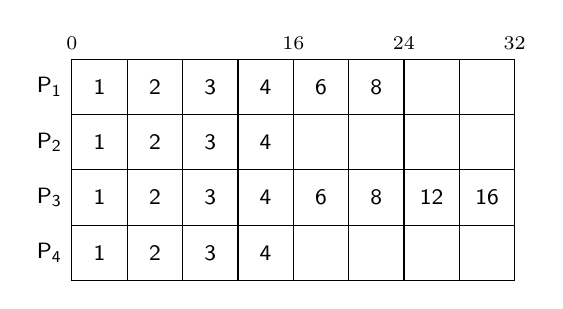
\begin{tikzpicture}

        %% \fill [black!80] (0,0) rectangle (14em, 2em);

        %% \fill [black!60] (14em,0) rectangle (22em, 2em);

        %% \fill [black!40] (22em,0) rectangle (24em, 2em);

        %% \fill [black!20] (24em,0) rectangle (32em, 2em);

        \draw (0,0) rectangle (16em,8em);

        \foreach \i in {1,...,7} {
          \draw [shorten >=0] (\i * 2em, 0) -- (\i * 2em, 8em);
        }

        \foreach \i in {1,...,3} {
          \draw [shorten >=0] (0, \i * 2em) -- (16em, \i * 2em);
        }

        \node [anchor=east] at (0, 7em) {\footnotesize $\mathsf{P_1}$};
        \node [anchor=east] at (0, 5em) {\footnotesize $\mathsf{P_2}$};
        \node [anchor=east] at (0, 3em) {\footnotesize $\mathsf{P_3}$};
        \node [anchor=east] at (0, 1em) {\footnotesize $\mathsf{P_4}$};

        \node at (1em, 7em) {\footnotesize $\mathsf{1}$};
        \node at (1em, 5em) {\footnotesize $\mathsf{1}$};
        \node at (1em, 3em) {\footnotesize $\mathsf{1}$};
        \node at (1em, 1em) {\footnotesize $\mathsf{1}$};

        \node at (3em, 7em) {\footnotesize $\mathsf{2}$};
        \node at (3em, 5em) {\footnotesize $\mathsf{2}$};
        \node at (3em, 3em) {\footnotesize $\mathsf{2}$};
        \node at (3em, 1em) {\footnotesize $\mathsf{2}$};

        \node at (5em, 7em) {\footnotesize $\mathsf{3}$};
        \node at (5em, 5em) {\footnotesize $\mathsf{3}$};
        \node at (5em, 3em) {\footnotesize $\mathsf{3}$};
        \node at (5em, 1em) {\footnotesize $\mathsf{3}$};

        \node at (7em, 7em) {\footnotesize $\mathsf{4}$};
        \node at (7em, 5em) {\footnotesize $\mathsf{4}$};
        \node at (7em, 3em) {\footnotesize $\mathsf{4}$};
        \node at (7em, 1em) {\footnotesize $\mathsf{4}$};

        \node at (9em, 7em) {\footnotesize $\mathsf{6}$};
        \node at (9em, 3em) {\footnotesize $\mathsf{6}$};

        \node at (11em, 7em) {\footnotesize $\mathsf{8}$};
        \node at (11em, 3em) {\footnotesize $\mathsf{8}$};

        \node at (13em, 3em) {\footnotesize $\mathsf{12}$};

        \node at (15em, 3em) {\footnotesize $\mathsf{16}$};

        \node [anchor=south] at (0em, 8em) {\scriptsize 0};
        \node [anchor=south] at (8em, 8em) {\scriptsize 16};
        \node [anchor=south] at (12em, 8em) {\scriptsize 24};
        \node [anchor=south] at (16em, 8em) {\scriptsize 32};
      \end{tikzpicture}
    \end{center}
  \end{frame}

  \begin{frame}
    \frametitle{IFS is the Fairest but Impractical Policy}

    This policy is fair, every process gets an equal amount of CPU time

    \hspace{2em} Boosts interactivity, has the ideal response time

    \vspace{2em}

    However, this would perform way too many context switches

    \vspace{2em}

    You have to constantly scan all processes, which is $\mathsf{O(N)}$
  \end{frame}

  \begin{frame}
    \frametitle{Completely Fair Scheduler (CFS)}

    For each runnable process, assign it a ``virtual runtime''

    \hspace{2em} At each scheduling point where the process runs for time \texttt{t}

    \hspace{4em} Increase the virtual runtime by \texttt{t} $\mathsf{\times}$ weight (based on priority)

    \vspace{2em}

    The virtual runtime monotonically increases

    \hspace{2em} Scheduler selects the process based on the lowest virtual runtime

    \hspace{4em} Compute its dynamic time slice based on the IFS

    \vspace{2em}

    Allow the process to run, when the time slice ends repeat the process
  \end{frame}

  \begin{frame}
    \frametitle{CFS is Implemented with Red-Black Trees}

    A red-black tree is a self-balancing binary search tree

    \hspace{2em} Keyed by virtual runtime

    \hspace{4em} $\mathsf{O(lg N)}$ insert, delete, update

    \hspace{4em} $\mathsf{O(1)}$ find minimum

    \vspace{2em}

    The implementation uses a red-black tree with nanosecond granularity

    \hspace{2em} Doesn't need to guess the interactivity of a process

    \vspace{2em}

    CFS tends to favour I/O bound processes by default

    \hspace{2em} Small CPU bursts translate to a low virtual runtime

    \hspace{4em} It will get a larger time slice, in order to catch up to the ideal
  \end{frame}

  \begin{frame}
    \frametitle{Scheduling Gets Even More Complex}

    There are more solutions, and more issues:
    \begin{itemize}
      \item Introducing priority also introduces priority inversion
      \item Some processes need good interactivity, others not so much
      \item Multiprocessors may require per-CPU queues
      \item Real-time requires predictability
      \item Completely Fair Scheduler (CFS) tries to model the ideal fairness
    \end{itemize}
  \end{frame}
\end{document}
